\documentclass[11pt]{article}

\usepackage[margin=1in]{geometry}
\usepackage[utf8]{inputenc}
\usepackage{amsmath,amssymb,amsfonts}
\usepackage{graphicx}
\usepackage{booktabs}
\usepackage{hyperref}
\usepackage{caption}
\usepackage{subcaption}
\usepackage{siunitx}
\usepackage{xcolor}
\usepackage{setspace}

\graphicspath{{figures/}}

\hypersetup{
  colorlinks=true,
  linkcolor=blue,
  citecolor=blue,
  urlcolor=blue
}

\sisetup{
  round-mode=places,
  round-precision=3,
  detect-all
}

\title{Online Resource 1\\Supplementary Material for\\
Semantic Action Landscapes: A Stochastic Least-Action Model Links Category Structure to Dynamic Response Competition}

\author{%
Antonio Pereira\\[0.4em]
\parbox{0.82\textwidth}{\centering
Signal Processing Laboratory\\
Universidade Federal do Par\'a (UFPA)\\
66075-110 Bel\'em, PA, Brazil\\
Corresponding author: \href{mailto:apereira@ufpa.br}{apereira@ufpa.br}}}

\date{}

\begin{document}

\maketitle

\noindent\textbf{Article title:} Semantic Action Landscapes: A Stochastic Least-Action Model Links Category Structure to Dynamic Response Competition

\noindent\textbf{Journal:} Computational Brain \& Behavior

\noindent\textbf{Author:} Antonio Pereira

\noindent\textbf{Corresponding author:} \href{mailto:apereira@ufpa.br}{apereira@ufpa.br}

\vspace{1em}

\doublespacing

\setcounter{table}{0}
\renewcommand{\thetable}{S\arabic{table}}
\setcounter{figure}{0}
\renewcommand{\thefigure}{S\arabic{figure}}
\setcounter{section}{0}
\renewcommand{\thesection}{S\arabic{section}}

\section*{Supplementary Material}

\section{Semantic Predictor Provenance}
\label{sec:supp-semantic-provenance}

The primary semantic predictor is the inverse-typicality margin computed from the item--category scoring table reported in the main text (Section~2.4). An independent published norm source mapping the exact 19 German animal exemplars to the same target and competitor categories was not identified. The semantic-margin analysis is therefore retrospective, and prospective validation with preregistered norms is the key next test.

Table~\ref{tab:semantic-provenance} compares the primary inverse-typicality margin with an ordinal robustness check based on within-condition semantic rank. The within-condition rank ordering preserves the relative ordering of items within each condition but does not constitute an independent norm source. Both orderings predict item-level $\hat{\rho}$ in the same direction.

\begin{table}[htbp]
\centering
\small
\caption{Semantic predictor provenance and ordinal robustness check. The primary predictor is the inverse-typicality margin from the item--category scoring table reported in the manuscript. An independent norm source for the exact 19 item--category pairs was not identified.}
\label{tab:semantic-provenance}
\begin{tabular}{lrrl}
\toprule
Source & Spearman with $\hat{\rho}$ & $p$ & Note \\
\midrule
Inverse-typicality margin (primary, this study) & -0.8548 & 3.152e-06 & Primary predictor; item--category scoring table reported in the manuscript \\
Within-condition rank ordering (ordinal robustness check) & -0.7250 & 4.444e-04 & Ordinal check only; not an independent norm source \\
\bottomrule
\end{tabular}
\end{table}


Table~\ref{tab:semantic-regression-details} reports the item-level regression details for the three semantic models, and Table~\ref{tab:semantic-loocv-metrics} reports leave-one-item-out semantic prediction metrics for fitted item-level $\rho$.

\begin{table}[htbp]
\centering
\small
\caption{Item-level semantic regression details for fitted competitor attraction.}
\label{tab:semantic-regression-details}
\begin{tabular}{llrlrrrrrrrrr}
\toprule
Model & Formula & Intercept & Term & Slope/statistic & SE & 95\% CI & $t$ & $p$ & $R^2$ & Adj. $R^2$ & AIC & $n$ items \\
\midrule
fitted $\rho$ $\sim$ atypical label & \texttt{rho\_hat ~ atypical} & 0.446 & atypical label & 0.242 & 0.054 & [0.128, 0.357] & 4.456 & 3.467e-04 & 0.539 & 0.512 & -28.004 & 19 \\
fitted $\rho$ $\sim$ semantic margin & \texttt{rho\_hat ~ semantic\_margin} & 0.650 & semantic margin & -0.546 & 0.068 & [-0.689, -0.404] & -8.078 & 3.196e-07 & 0.793 & 0.781 & -43.258 & 19 \\
fitted $\rho$ $\sim$ atypical label + semantic margin & \texttt{rho\_hat ~ atypical + semantic\_margin} & 0.712 & atypical label & -0.087 & 0.078 & [-0.254, 0.079] & -1.116 & 0.2811 & 0.808 & 0.784 & -42.681 & 19 \\
fitted $\rho$ $\sim$ atypical label + semantic margin & \texttt{rho\_hat ~ atypical + semantic\_margin} & 0.712 & semantic margin & -0.691 & 0.146 & [-0.999, -0.382] & -4.742 & 2.210e-04 & 0.808 & 0.784 & -42.681 & 19 \\
Pearson correlation & \texttt{rho\_hat vs semantic\_margin} & -- & $r$ & -0.891 & -- & [-0.958, -0.733] & -8.078 & 3.196e-07 & 0.793 & -- & -- & 19 \\
Spearman correlation & \texttt{rho\_hat vs semantic\_margin} & -- & $\rho_s$ & -0.855 & -- & -- & -- & 3.152e-06 & -- & -- & -- & 19 \\
\bottomrule
\end{tabular}
\end{table}


\begin{table}[htbp]
\centering
\caption{Leave-one-item-out semantic prediction metrics for fitted item-level $\rho$.}
\label{tab:semantic-loocv-metrics}
\begin{tabular}{lr}
\toprule
Metric & Value \\
\midrule
Pearson $r$ predicted vs observed $\rho$ & 0.838 \\
Pearson $p$ & 7.491e-06 \\
Spearman $\rho_s$ predicted vs observed $\rho$ & 0.847 \\
Spearman $p$ & 4.681e-06 \\
RMSE & 0.084 \\
MAE & 0.063 \\
Calibration intercept & 0.019 \\
Calibration slope & 0.969 \\
N items & 19 \\
Largest absolute residual item & Wal \\
Residual for that item & 0.240 \\
\bottomrule
\end{tabular}
\end{table}


\subsection{Multisource semantic validation}
\label{sec:supp-multisource}

A multisource semantic validation was conducted to test whether the semantic--action relation generalized beyond the reported item--category scoring table. An audit of published German semantic resources found no verified accessible typicality norm covering the exact 19 item--category contrasts (Table~\ref{tab:semantic-source-audit}). The secondary computational check therefore evaluated three pretrained multilingual sentence-embedding models: \texttt{T-Systems-onsite/cross-en-de-roberta-sentence-transformer}, \texttt{paraphrase-multilingual-mpnet-base-v2}, and \texttt{multilingual-e5-base}. German animal names and category labels were encoded after transliterated umlauts were corrected to canonical orthography, for example \textit{Saeugetier} $\rightarrow$ \textit{Säugetier} and \textit{Chamaeleon} $\rightarrow$ \textit{Chamäleon}. Embedding margins were computed as $\mathrm{emb\_margin}_i = \mathrm{emb\_sim}_{T,i} - \mathrm{emb\_sim}_{C,i}$. A rank-averaged multisource margin was also computed across the three embedding models.

The main-text multisource validation table summarizes the validation metrics. After orthographic correction, the rank-averaged embedding margin predicted fitted and held-out item-level $\hat{\rho}$. These results show that the semantic--action relation is recoverable from independent computational representations and is not confined to the reported scoring table. Table~\ref{tab:multisource-semantic-scores} reports the item-level scores across all evaluated sources.

\begin{table}[htbp]
\centering
\caption{Audit of German semantic resources evaluated for prospective validation.}
\label{tab:semantic-source-audit}
\resizebox{\linewidth}{!}{%
\begin{tabular}{p{3.5cm}llcp{5cm}}
\toprule
Source & Type & Access & Cov. & Reason for inclusion/exclusion \\
\midrule
Battig \& Montague (1969) & Category norms & Available & 0/19 & English only \\
Rosch (1975) & Typicality norms & Available & 0/19 & English only \\
Mannhaupt (1983) & Category norms & Not freely accessible & 0/19 & Requires library access, unlikely to cover exact contrasts \\
SWOW-DE & Free association & Available & 0/19 & Uncertain coverage for exact 19 item-category roles without manual processing \\
GermaNet & Lexical database & Registration required & 0/19 & Requires institutional registration, not freely downloadable \\
SUBTLEX-DE & Word frequency & Available & 19/19 & Useful only as covariate, not as semantic margin \\
\bottomrule
\end{tabular}
}%
\end{table}


\begin{table}[htbp]
\centering
\caption{Item-level scores across all valid semantic sources.}
\label{tab:multisource-semantic-scores}
\resizebox{\linewidth}{!}{%
\begin{tabular}{llccccccccc}
\toprule
Item & Cond. & Tgt & Comp & $\hat{\rho}$ & Prim. & MiniLM & MPNet & DistilUSE & E5 & RankMean \\
\midrule
Wal & Aty & Saeu & Fisc & 0.98 & -0.30 & -0.04 & -0.36 & 0.04 & -0.05 & 5.00 \\
Fledermaus & Aty & Saeu & Voge & 0.72 & -0.14 & 0.00 & 0.03 & 0.13 & -0.01 & 10.75 \\
Pinguin & Aty & Voge & Fisc & 0.70 & -0.10 & -0.26 & -0.08 & 0.10 & -0.02 & 5.50 \\
Seeloewe & Aty & Saeu & Fisc & 0.63 & -0.10 & 0.01 & 0.22 & 0.18 & 0.06 & 15.50 \\
Schmetterling & Aty & Inse & Voge & 0.59 & -0.03 & -0.13 & 0.42 & 0.13 & -0.02 & 11.25 \\
Aal & Aty & Fisc & Rept & 0.50 & 0.10 & -0.19 & 0.02 & 0.04 & -0.01 & 6.75 \\
Klapperschlange & Typ & Rept & Amph & 0.63 & 0.18 & 0.15 & 0.11 & 0.10 & 0.01 & 13.25 \\
Chamaeleon & Typ & Rept & Inse & 0.41 & 0.26 & 0.14 & 0.01 & 0.08 & 0.01 & 11.50 \\
Spatz & Typ & Voge & Saeu & 0.56 & 0.29 & 0.06 & -0.07 & -0.22 & 0.04 & 9.25 \\
Lachs & Typ & Fisc & Saeu & 0.48 & 0.30 & 0.04 & -0.09 & -0.08 & 0.06 & 9.50 \\
Alligator & Typ & Rept & Saeu & 0.41 & 0.31 & 0.11 & 0.43 & 0.29 & 0.07 & 18.00 \\
Hai & Typ & Fisc & Saeu & 0.45 & 0.35 & -0.08 & -0.15 & -0.07 & 0.03 & 7.00 \\
Falke & Typ & Voge & Rept & 0.44 & 0.38 & -0.23 & 0.14 & 0.11 & -0.00 & 10.00 \\
Goldfisch & Typ & Fisc & Amph & 0.37 & 0.40 & 0.45 & 0.30 & 0.25 & 0.05 & 17.50 \\
Kaninchen & Typ & Saeu & Rept & 0.39 & 0.44 & -0.12 & -0.09 & -0.14 & -0.03 & 3.75 \\
Loewe & Typ & Saeu & Fisc & 0.49 & 0.48 & 0.28 & 0.21 & 0.10 & 0.02 & 14.50 \\
Pferd & Typ & Saeu & Voge & 0.42 & 0.52 & 0.02 & 0.10 & -0.01 & -0.08 & 7.50 \\
Katze & Typ & Saeu & Rept & 0.37 & 0.52 & -0.22 & -0.07 & -0.09 & -0.01 & 5.25 \\
Hund & Typ & Saeu & Inse & 0.38 & 0.57 & -0.01 & 0.13 & 0.07 & -0.06 & 8.25 \\
\bottomrule
\end{tabular}
}%
\end{table}


\section{Path and Negative-Control Analyses}
\label{sec:supp-path-negative-controls}

The main text reports the item-level path model because semantic margin varies at the item level. Table~\ref{tab:path-mediation-trial} reports the complementary trial-level mixed path estimates. These models used subject grouping with an item variance component and asked whether semantic margin predicted behavioral outcomes indirectly through fitted $\hat{\rho}$.

\begin{table}[htbp]
\centering
\small
\caption{Trial-level path estimates for the semantic margin $\rightarrow \rho \rightarrow$ behavior chain. Fixed effects come from mixed models with subject grouping and an item variance component.}
\label{tab:path-mediation-trial}
\resizebox{\linewidth}{!}{%
\begin{tabular}{lrrrrrr}
\toprule
Outcome & $a$: margin $\rightarrow \rho$ & $b$: $\rho \rightarrow$ outcome & Indirect $a b$ & Total margin effect & Direct margin effect & \% indirect \\
\midrule
AUC & -0.536 & 0.351 & -0.188 & -0.163 & 0.025 & 115.351 \\
Maximum deviation & -0.536 & 0.919 & -0.492 & -0.492 & 0.001 & 100.115 \\
Response time & -0.536 & 0.165 & -0.088 & -1.768 & -1.679 & 4.993 \\
\bottomrule
\end{tabular}
}%
\end{table}


Table~\ref{tab:negative-control-semantics} reports the targeted semantic negative-control analysis. The reversed margin is included as an orientation diagnostic rather than as an independent predictor, because an unconstrained linear model can reverse its slope and recover the same numerical fit. The theoretically relevant point is that it fails the prespecified sign test.

\begin{table}[htbp]
\centering
\small
\caption{Targeted semantic negative controls. NLL gain is item-weighted condition-only action NLL minus predictor-based action NLL; positive values favor the predictor.}
\label{tab:negative-control-semantics}
\resizebox{\linewidth}{!}{%
\begin{tabular}{llrrlrrrl}
\toprule
Predictor & Role & Slope & $R^2$ & Direction ok & Mean NLL & NLL gain & Improved items & Null/notes \\
\midrule
Real target--competitor margin & Primary semantic contrast & -0.546 & 0.793 & Yes & 39.171 & 0.694 & 15 & primary \\
Reversed competitor--target margin & Orientation control & 0.546 & 0.793 & No & 39.171 & 0.694 & 15 & algebraic mirror; sign fails \\
Target similarity alone & Component control & -0.758 & 0.674 & Yes & 39.336 & 0.528 & 15 & single component \\
Competitor similarity alone & Component control & 1.494 & 0.841 & Yes & 39.138 & 0.726 & 17 & single component \\
Word length & Lexical control & 0.003 & 0.003 & n/a & 39.943 & -0.079 & 8 & nonsemantic \\
Atypical label & Condition label & 0.242 & 0.539 & Yes & 39.864 & 0.000 & 0 & condition reference \\
Permuted margins & Permutation control & -- & -- & n/a & -- & -0.016 & -- & empirical $p = 2.0\times 10^{-4}$; 5000 draws \\
Random competitor-score assignment & Competitor assignment control & -- & -- & n/a & -- & 0.416 & -- & null $p = 0.007$; 5000 draws \\
\bottomrule
\end{tabular}
}%
\end{table}


\section{Item-Level Uncertainty}
\label{sec:supp-item-uncertainty}

\subsection{Bootstrap confidence interval for mean NLL gain}

Because semantic margin varies across only 19 items, item-level inference is primary. The mean item-wise NLL gain of 0.694 units was evaluated by item-resampling bootstrap with 4,000 replications. The 95\% bootstrap confidence interval for the mean item-wise gain was [0.230, 1.384] NLL units, computed by the percentile method. The gain was positive for 15 of 19 items; an exact two-tailed binomial sign test against $H_0: p = 0.5$ yielded $p = 0.019$.

\begin{table}[htbp]
\centering
\caption{Item-level NLL gain: bootstrap CI and sign test.}
\label{tab:item-bootstrap}
\begin{tabular}{lr}
\toprule
Statistic & Value \\
\midrule
N items & 19 \\
N items with positive gain & 15 \\
Mean NLL gain & 0.694 \\
Bootstrap 95\% CI lower & 0.230 \\
Bootstrap 95\% CI upper & 1.384 \\
Sign test $p$ & 0.019 \\
\bottomrule
\end{tabular}
\end{table}


\subsection{Leave-one-item-out residuals}

Table~\ref{tab:loocv-residuals} reports the leave-one-item-out residuals, defined as $\hat{\rho}_{\mathrm{obs}} - \hat{\rho}_{\mathrm{sem}}$, for each of the 19 items. Positive residuals indicate that the semantic model underpredicted the item's fitted $\rho$, meaning that the item showed more competitor attraction than its semantic margin predicted. The largest positive residual was observed for Wal, which had the most negative semantic margin and the highest fitted $\rho$ in the dataset.

\begin{table}[htbp]
\centering
\caption{Leave-one-item-out LOOCV residuals for the semantic-prior $\rho$ model.}
\label{tab:loocv-residuals}
\begin{tabular}{lrrrr}
\toprule
Item & Condition & rho obs & rho sem & Residual \\
\midrule
Aal & Atypical & 0.500 & 0.600 & -0.100 \\
Alligator & Typical & 0.412 & 0.482 & -0.070 \\
Chamaeleon & Typical & 0.406 & 0.512 & -0.106 \\
Falke & Typical & 0.439 & 0.443 & -0.004 \\
Fledermaus & Atypical & 0.723 & 0.725 & -0.002 \\
Goldfisch & Typical & 0.373 & 0.437 & -0.063 \\
Hai & Typical & 0.446 & 0.461 & -0.015 \\
Hund & Typical & 0.384 & 0.331 & 0.053 \\
Kaninchen & Typical & 0.388 & 0.411 & -0.024 \\
Katze & Typical & 0.373 & 0.364 & 0.009 \\
Klapperschlange & Typical & 0.626 & 0.550 & 0.076 \\
Lachs & Typical & 0.480 & 0.486 & -0.007 \\
Loewe & Typical & 0.492 & 0.374 & 0.118 \\
Pferd & Typical & 0.417 & 0.358 & 0.059 \\
Pinguin & Atypical & 0.699 & 0.706 & -0.007 \\
Schmetterling & Atypical & 0.594 & 0.676 & -0.082 \\
Seeloewe & Atypical & 0.629 & 0.715 & -0.085 \\
Spatz & Typical & 0.560 & 0.490 & 0.069 \\
Wal & Atypical & 0.983 & 0.743 & 0.240 \\
\bottomrule
\end{tabular}
\end{table}

\subsection{Item-level influence analysis}

Table~\ref{tab:item-influence} reports the mean NLL gain after excluding each item one at a time. If the overall gain were driven by one atypical item, removing that item would substantially reduce the gain. Excluding Wal produced the largest reduction in the mean gain, whereas excluding typical items with near-zero gain left the result closer to the full-sample estimate. The gain is therefore influenced by the most competitive atypical items, but it is not driven exclusively by a single outlier item.

\begin{table}[htbp]
\centering
\caption{Item-level influence: mean NLL gain (semantic vs.\ condition) after excluding each item one at a time.}
\label{tab:item-influence}
\begin{tabular}{lrr}
\toprule
excluded\_item & mean\_nll\_gain\_without & n\_remaining \\
\midrule
Wal & 0.4039 & 18 \\
Klapperschlange & 0.6328 & 18 \\
Fledermaus & 0.6514 & 18 \\
Spatz & 0.6673 & 18 \\
Pinguin & 0.6877 & 18 \\
Lachs & 0.7082 & 18 \\
Loewe & 0.7097 & 18 \\
Hai & 0.7173 & 18 \\
Katze & 0.7178 & 18 \\
Falke & 0.7182 & 18 \\
Hund & 0.7193 & 18 \\
Pferd & 0.7205 & 18 \\
Kaninchen & 0.7229 & 18 \\
Goldfisch & 0.7231 & 18 \\
Alligator & 0.7249 & 18 \\
Chamaeleon & 0.7343 & 18 \\
Seeloewe & 0.7353 & 18 \\
Schmetterling & 0.7361 & 18 \\
Aal & 0.7469 & 18 \\
\bottomrule
\end{tabular}
\end{table}

Table~\ref{tab:item-slope-influence-summary} and Table~\ref{tab:item-slope-influence} report the corresponding jackknife influence analysis for the semantic margin $\rightarrow \hat{\rho}$ slope. All jackknife slopes remained negative, and removing Wal produced the largest attenuation.

\begin{table}[htbp]
\centering
\caption{Item-level semantic slope influence summary.}
\label{tab:item-slope-influence-summary}
\begin{tabular}{lr}
\toprule
Statistic & Value \\
\midrule
Full OLS slope & -0.546 \\
Full OLS p & $<.001$ \\
Jackknife slope min & -0.571 \\
Jackknife slope max & -0.439 \\
All jackknife slopes negative & Yes \\
Bootstrap slope CI lower & -0.699 \\
Bootstrap slope CI upper & -0.362 \\
Full Spearman & -0.855 \\
Bootstrap Spearman CI lower & -0.969 \\
Bootstrap Spearman CI upper & -0.570 \\
Theil-Sen slope & -0.482 \\
Theil-Sen CI lower & -0.652 \\
Theil-Sen CI upper & -0.342 \\
\bottomrule
\end{tabular}
\end{table}


\begin{table}[htbp]
\centering
\small
\caption{Leave-one-item-out influence on the item-level semantic margin slope.}
\label{tab:item-slope-influence}
\resizebox{\linewidth}{!}{%
\begin{tabular}{lrrrr}
\toprule
Excluded item & Slope without item & Slope p & Spearman & Spearman p \\
\midrule
Loewe & -0.571 & $<.001$ & -0.899 & $<.001$ \\
Seeloewe & -0.570 & $<.001$ & -0.829 & $<.001$ \\
Schmetterling & -0.565 & $<.001$ & -0.833 & $<.001$ \\
Hund & -0.561 & $<.001$ & -0.843 & $<.001$ \\
Pferd & -0.561 & $<.001$ & -0.878 & $<.001$ \\
Aal & -0.557 & $<.001$ & -0.839 & $<.001$ \\
Spatz & -0.549 & $<.001$ & -0.850 & $<.001$ \\
Katze & -0.549 & $<.001$ & -0.839 & $<.001$ \\
Pinguin & -0.548 & $<.001$ & -0.829 & $<.001$ \\
Fledermaus & -0.547 & $<.001$ & -0.829 & $<.001$ \\
Lachs & -0.546 & $<.001$ & -0.856 & $<.001$ \\
Falke & -0.546 & $<.001$ & -0.862 & $<.001$ \\
Hai & -0.545 & $<.001$ & -0.862 & $<.001$ \\
Chamaeleon & -0.544 & $<.001$ & -0.898 & $<.001$ \\
Klapperschlange & -0.543 & $<.001$ & -0.837 & $<.001$ \\
Kaninchen & -0.542 & $<.001$ & -0.859 & $<.001$ \\
Alligator & -0.542 & $<.001$ & -0.876 & $<.001$ \\
Goldfisch & -0.538 & $<.001$ & -0.867 & $<.001$ \\
Wal & -0.439 & $<.001$ & -0.829 & $<.001$ \\
\bottomrule
\end{tabular}
}%
\end{table}


\begin{figure}[htbp]
  \centering
  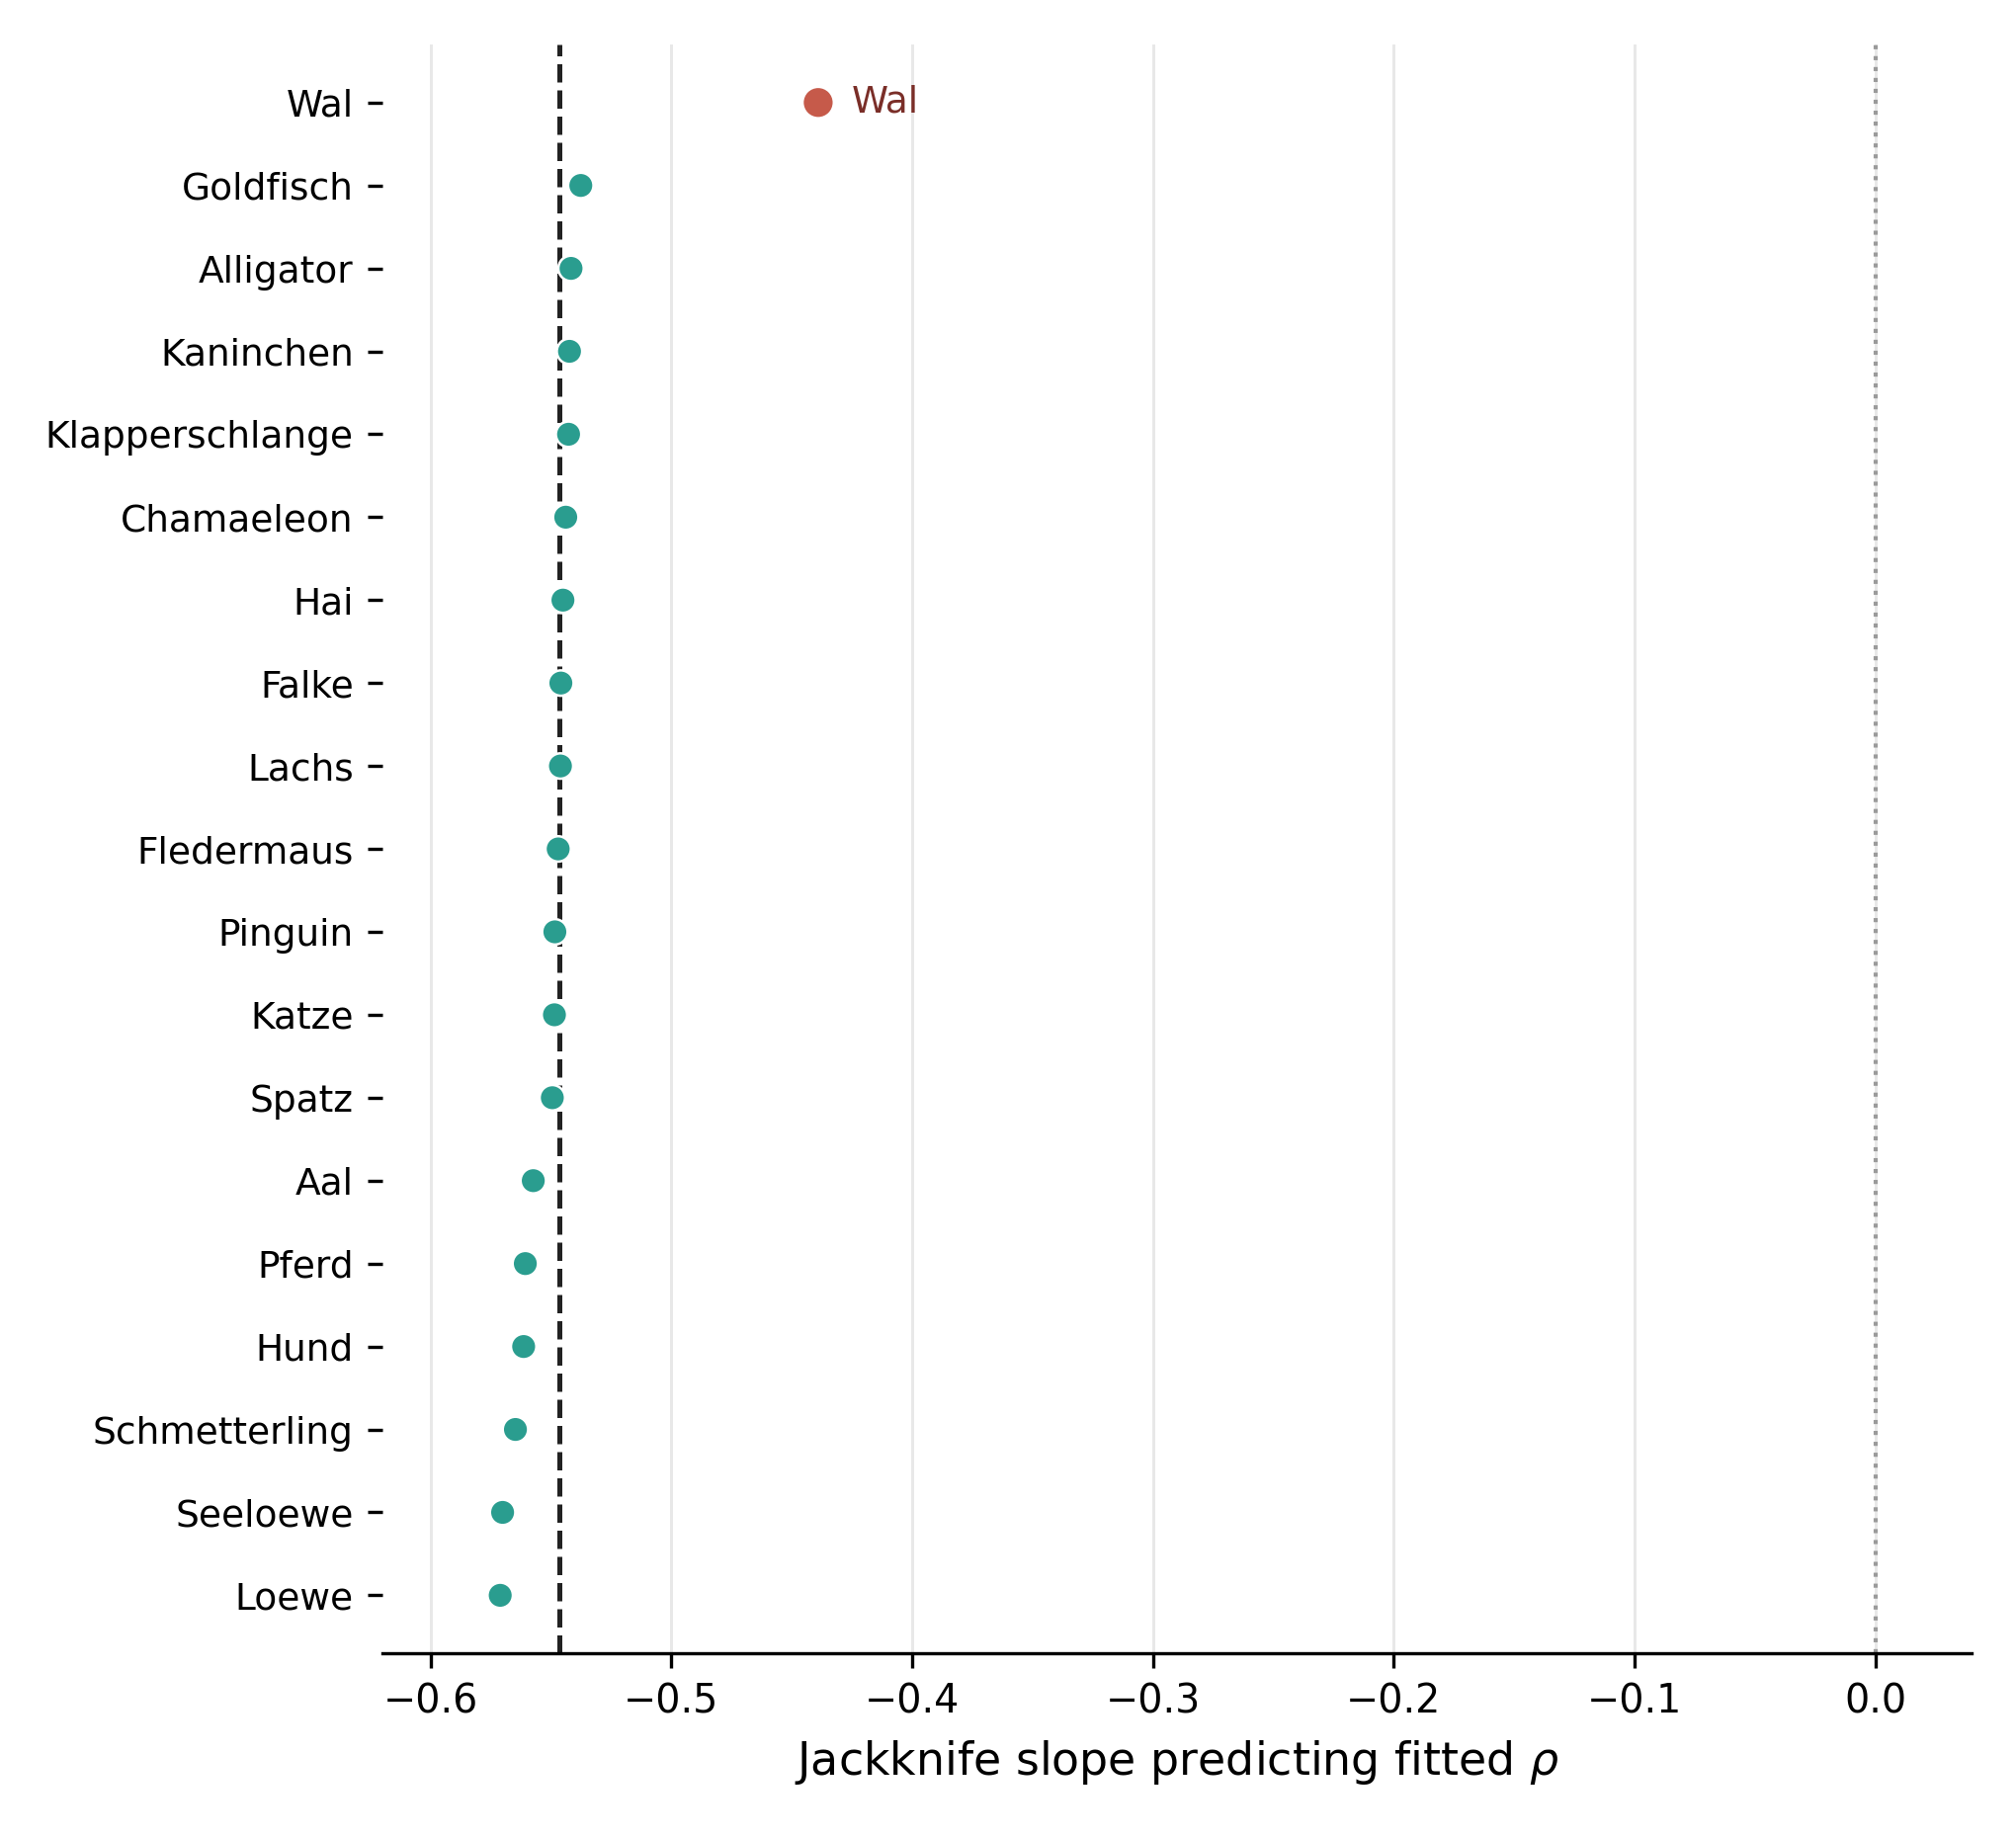
\includegraphics[width=0.86\linewidth]{semantic_slope_jackknife.png}
  \caption{\textbf{Leave-one-item-out semantic slope influence.} The margin--$\rho$ slope was recomputed after excluding each exemplar in turn. All slopes remained negative. Removing Wal produced the largest attenuation, but the estimated slope remained below zero.}
  \label{fig:supp-semantic-slope-jackknife}
\end{figure}

\section{Subject-Wise Cross-Validation}
\label{sec:supp-subject-cv}

Table~\ref{tab:subject-cv-paired} reports paired subject-level RMSE comparisons for the subject-wise cross-validation analysis. The paired difference is defined as minimum-jerk RMSE minus action-model RMSE, so positive values indicate lower RMSE for the action model.

\begin{table}[htbp]
\centering
\small
\caption{Subject-wise cross-validation paired RMSE comparisons.}
\label{tab:subject-cv-paired}
\begin{tabular}{lrrrrlrr}
\toprule
Condition & Mean RMSE action & Mean RMSE minimum jerk & Minimum jerk -- action & 95\% bootstrap CI & Test & $p$ & $n$ subjects \\
\midrule
All trials & 0.461 & 0.481 & 0.020 & [0.017, 0.022] & paired $t$ & 5.332e-22 & 60 \\
Typical trials & 0.433 & 0.449 & 0.015 & [0.014, 0.017] & paired $t$ & 2.108e-23 & 60 \\
Atypical trials & 0.528 & 0.557 & 0.029 & [0.023, 0.035] & paired $t$ & 3.950e-13 & 60 \\
\bottomrule
\end{tabular}
\end{table}


\section{Parameter Boundary Report}
\label{sec:supp-boundary}

The competitor-attraction grid covered $\rho \in [0.00, 2.00]$ in steps of 0.05, giving 41 grid points. Table~\ref{tab:boundary-report} reports the percentage of trial-level, item-level, and fold-level fits at the grid boundaries. Approximately 7.0\% of trial-level fits were at $\rho = 0.00$ and 3.4\% were at $\rho = 2.00$. Because fewer than 15\% of trial-level fits reached the upper boundary, the current grid range is adequate for the majority of trials. No item-level mean fit reached either boundary. The $\rho = 2.00$ boundary affects a minority of atypical trials, primarily Wal; expanding the grid to $\rho_{\max} = 3.00$ or using continuous optimization is recommended for future work with more extreme items.

\begin{table}[htbp]
\centering
\caption{Parameter boundary report: percentage of fits at $\rho = 0$ or $\rho = 2.00$.}
\label{tab:boundary-report}
\begin{tabular}{lrrr}
\toprule
Level & Boundary & N & Pct \\
\midrule
Trial & rho=0.00 & 75 & 7.0\% \\
Trial & rho=2.00 & 36 & 3.4\% \\
Trial & Either & 111 & 10.4\% \\
Item & Either & 0 & 0.0\% \\
Fold & Either & 0 & 0.0\% \\
\bottomrule
\end{tabular}
\end{table}

\section{Sensitivity for \texorpdfstring{$\lambda$}{lambda} and \texorpdfstring{$\gamma$}{gamma}}
\label{sec:supp-lambda-gamma}

The primary sensitivity table in the main text varies $\alpha$, $\beta$, $\sigma_C$, and $K$. Table~\ref{tab:sensitivity-lambda-gamma} documents the analytical effect of perturbing $\lambda$, the potential scale, and $\gamma$, the competitor-decay exponent.

Full empirical sensitivity for $\lambda$ and $\gamma$ requires recomputing the action grid because these parameters appear inside the action functional. The key identifiability constraint is that $\lambda$ and $\rho$ are multiplicatively coupled in the potential term. Rescaling $\lambda$ by a constant $c$ shifts all fitted $\hat{\rho}$ values by approximately $1/c$, so the sign of the semantic-margin slope is preserved but the numerical slope changes. Changing $\gamma$ shifts the temporal profile of competitor attraction without altering the overall $\lambda \cdot \rho$ product. Neither perturbation is expected to change the sign of the margin--$\rho$ relationship, which is the primary claim of the semantic analysis.

\begin{table}[htbp]
\centering
\caption{Sensitivity of $\hat{\rho}$ and the semantic-margin slope to $\lambda$ and $\gamma$. Full recomputation of the action grid for perturbed $\lambda$ and $\gamma$ is not reported because the $\lambda$--$\rho$ scale confound means only the sign of the semantic slope is identifiable without path recomputation.}
\label{tab:sensitivity-lambda-gamma}
\begin{tabular}{lrrrr}
\toprule
Parameter & Perturbation & Effect on fitted $\rho$ & Semantic slope direction & Source \\
\midrule
$\lambda$ & $\times 0.5$ & $\hat{\rho} \approx 2\hat{\rho}\_0$ (scale confound) & Unchanged (negative) & Analytical \\
$\lambda$ & $\times 1.0$ (baseline) & --- & Negative (observed) & Empirical \\
$\lambda$ & $\times 2.0$ & $\hat{\rho} \approx 0.5\hat{\rho}\_0$ (scale confound) & Unchanged (negative) & Analytical \\
$\gamma$ & $\times 0.5$ & Competitor attraction earlier in trajectory & Unchanged (negative) & Analytical \\
$\gamma$ & $\times 1.0$ (baseline) & --- & Negative (observed) & Empirical \\
$\gamma$ & $\times 2.0$ & Competitor attraction more concentrated at start & Unchanged (negative) & Analytical \\
\bottomrule
\end{tabular}
\end{table}

\section{Residual and Noise Robustness}
\label{sec:supp-robustness}

The primary NLL model assumes independent isotropic Gaussian residuals around the model path. Table~\ref{tab:stochastic-variance-calibration} reports the fold-level training variance estimates used in the stochastic likelihood calculation. Table~\ref{tab:robustness-rmse} provides an RMSE-only item-level comparison that does not require the Gaussian likelihood assumption. In terms of raw RMSE, the condition-only action model achieves lower item-mean error than the semantic-margin model for 15 of 19 items. The NLL gain for 15 of 19 items under the stochastic model therefore arises from residual-variance calibration in the leave-one-item-out fold rather than uniformly lower raw RMSE.

\begin{table}[htbp]
\centering
\small
\caption{Training residual variance and held-out fit for stochastic trajectory likelihood models. Variance entries are mean fold-level $\tau^2$ with range in brackets.}
\label{tab:stochastic-variance-calibration}
\begin{tabular}{lrrrrrl}
\toprule
Model & Training $\tau^2$ & Residual SD $\tau$ & Held-out RMSE & Held-out NLL & $n$ trials & Variance estimate \\
\midrule
condition-only action $\rho$ & 0.1248 [0.1200, 0.1273] & 0.353 & 0.461 & 38.813 & 1064 & by fold and model \\
semantic-margin action $\rho$ & 0.1231 [0.1190, 0.1255] & 0.351 & 0.462 & 38.175 & 1064 & by fold and model \\
condition + semantic action $\rho$ & 0.1231 [0.1190, 0.1255] & 0.351 & 0.462 & 38.219 & 1064 & by fold and model \\
trial-fitted $\rho$ upper bound & 0.1080 [0.1052, 0.1099] & 0.329 & 0.435 & 31.386 & 1064 & by fold and model \\
minimum jerk & 0.1387 [0.1324, 0.1416] & 0.372 & 0.480 & 44.294 & 1064 & by fold and model \\
\bottomrule
\end{tabular}
\end{table}


\begin{table}[htbp]
\centering
\caption{RMSE-only item-level robustness check (no iid Gaussian assumption required). The condition-only action model had lower item-mean RMSE than the semantic-margin model for 15 of 19 items (sign test against H$_0$: no difference, $p = 0.019$). The NLL gain for 15/19 items under the full stochastic model reflects better variance (\(\tau^2\)) calibration in the leave-one-item-out fold rather than lower raw RMSE.}
\label{tab:robustness-rmse}
\begin{tabular}{lrr}
\toprule
Item & RMSE gain (Cond--Sem) & Lower RMSE model \\
\midrule
Aal & -0.0029 & Condition \\
Alligator & -0.0031 & Condition \\
Chamaeleon & -0.0048 & Condition \\
Falke & -0.0004 & Condition \\
Fledermaus & -0.0001 & Condition \\
Goldfisch & -0.0016 & Condition \\
Hai & -0.0017 & Condition \\
Hund & 0.0000 & Condition \\
Kaninchen & -0.0011 & Condition \\
Katze & 0.0000 & Condition \\
Klapperschlange & 0.0003 & Semantic \\
Lachs & -0.0002 & Condition \\
Loewe & 0.0002 & Semantic \\
Pferd & 0.0000 & Condition \\
Pinguin & -0.0047 & Condition \\
Schmetterling & -0.0039 & Condition \\
Seeloewe & -0.0088 & Condition \\
Spatz & 0.0031 & Semantic \\
Wal & 0.0138 & Semantic \\
\bottomrule
\end{tabular}
\end{table}

\section{Error-Trial Analysis}
\label{sec:supp-error}

The main trajectory analysis excluded incorrect trials because the action model was defined for correct target-directed paths after canonicalization. Table~\ref{tab:error-by-condition} reports error counts and rates by condition. Atypical items produced substantially higher error rates than typical items, consistent with response competition. Table~\ref{tab:error-by-item} reports error counts by item. The three highest-error items, Fledermaus, Wal, and Klapperschlange, all had below-average semantic margins.

\begin{table}[htbp]
\centering
\caption{Error counts and rates by condition.}
\label{tab:error-by-condition}
\begin{tabular}{lrrr}
\toprule
Condition & N Trials & N Errors & Error Rate \\
\midrule
Atypical & 360 & 40 & 0.111 \\
Typical & 780 & 36 & 0.046 \\
\bottomrule
\end{tabular}
\end{table}

\begin{table}[htbp]
\centering
\caption{Error counts and rates by item (all trials).}
\label{tab:error-by-item}
\begin{tabular}{lrrr}
\toprule
Item & N Trials & N Errors & Error Rate \\
\midrule
Fledermaus & 60 & 17 & 0.283 \\
Klapperschlange & 60 & 14 & 0.233 \\
Wal & 60 & 9 & 0.150 \\
Hai & 60 & 9 & 0.150 \\
Seeloewe & 60 & 5 & 0.083 \\
Aal & 60 & 5 & 0.083 \\
Pinguin & 60 & 3 & 0.050 \\
Spatz & 60 & 3 & 0.050 \\
Katze & 60 & 3 & 0.050 \\
Alligator & 60 & 2 & 0.033 \\
Falke & 60 & 2 & 0.033 \\
Chamaeleon & 60 & 2 & 0.033 \\
Lachs & 60 & 1 & 0.017 \\
Schmetterling & 60 & 1 & 0.017 \\
Goldfisch & 60 & 0 & 0.000 \\
Hund & 60 & 0 & 0.000 \\
Kaninchen & 60 & 0 & 0.000 \\
Loewe & 60 & 0 & 0.000 \\
Pferd & 60 & 0 & 0.000 \\
\bottomrule
\end{tabular}
\end{table}

Table~\ref{tab:error-logistic} reports a compact logistic regression predicting trial-level errors from semantic margin and condition. Table~\ref{tab:error-logistic-details} adds odds ratios, odds-ratio confidence intervals, sample size, error count, pseudo-$R^2$, and standard-error type.

\begin{table}[htbp]
\centering
\caption{Logistic regression: error $\sim$ semantic margin + condition.}
\label{tab:error-logistic}
\begin{tabular}{lrrr}
\toprule
Predictor & Coefficient & SE & p \\
\midrule
Intercept & -1.0141 & 0.3948 & 0.0102 \\
semantic\_margin & -5.7149 & 1.1024 & $<.001$ \\
atypical & -1.7728 & 0.5775 & 0.0021 \\
\bottomrule
\end{tabular}
\end{table}


\begin{table}[htbp]
\centering
\small
\caption{Logistic regression details for trial-level errors.}
\label{tab:error-logistic-details}
\begin{tabular}{lrrrrrrrrl}
\toprule
Term & Coefficient & SE & $p$ & Odds ratio & OR 95\% CI & $n$ trials & $n$ errors & McFadden $R^2$ & SE type \\
\midrule
intercept & -1.0141 & 0.3948 & 0.0102 & 0.363 & [0.167, 0.786] & 1140 & 76 & 0.080 & conventional MLE \\
semantic margin & -5.7149 & 1.1024 & 2.170e-07 & 0.003 & [0.000, 0.029] & 1140 & 76 & 0.080 & conventional MLE \\
atypical label & -1.7728 & 0.5775 & 0.0021 & 0.170 & [0.055, 0.527] & 1140 & 76 & 0.080 & conventional MLE \\
\bottomrule
\end{tabular}
\end{table}


\section{Covariate Sensitivity}
\label{sec:supp-covariate}

With only 19 items, a large multiple regression is not appropriate. Table~\ref{tab:covariate-sensitivity} reports one-covariate-at-a-time checks for the semantic-margin slope in $\hat{\rho} \sim \mathrm{margin} + \mathrm{covariate}$. The semantic-margin slope remains negative across all covariate additions, indicating that the margin--$\hat{\rho}$ relationship is not explained by word length, item response time, number of trials, or typical/atypical label.

\begin{table}[htbp]
\centering
\caption{Covariate sensitivity: semantic-margin slope in $\hat{\rho} \sim \mathrm{margin} + \mathrm{covariate}$ (one covariate at a time, $n=19$ items).}
\label{tab:covariate-sensitivity}
\begin{tabular}{lrrrr}
\toprule
Covariate added & Semantic margin slope & Slope p & Slope sign negative & R2 \\
\midrule
(none – base model) & -0.5464 & $<.001$ & Yes & 0.7933 \\
word\_length & -0.5663 & $<.001$ & Yes & 0.8140 \\
raw\_rt\_s & -0.4425 & 0.0020 & Yes & 0.8066 \\
n\_trials & -0.4975 & $<.001$ & Yes & 0.8069 \\
atypical\_int & -0.6906 & $<.001$ & Yes & 0.8083 \\
\bottomrule
\end{tabular}
\end{table}


\section{Mixed-Effects Validation Details}
\label{sec:supp-mixed-effects}

Table~\ref{tab:mixed-effects-details} reports the exact mixed-effects model details for the trial-level validation. The fitted model used an item variance component with subject grouping in \texttt{statsmodels}; no separate subject random-intercept variance was estimated by this specification. This reporting preserves the fitted model used for the compact mixed-effects table rather than substituting a different estimator.

\begin{table}[htbp]
\centering
\small
\caption{Mixed-effects model details for trial-level $\rho$.}
\label{tab:mixed-effects-details}
\begin{tabular}{llrrrr}
\toprule
Component & Term/quantity & Value/coefficient & SE & 95\% CI & $p$ \\
\midrule
Model & Formula & \texttt{rho\_hat ~ semantic\_margin + atypical} & -- & -- & -- \\
Estimator/package & Estimator & statsmodels MixedLM, ML, L-BFGS & -- & -- & -- \\
Random effects & Included & item variance component with subject grouping; no subject random-intercept variance estimated & -- & -- & -- \\
Random effect variance & Subject & not estimated & -- & -- & -- \\
Random effect variance & Item & 0.096243 & -- & -- & -- \\
Residual variance & Residual & 0.096243 & -- & -- & -- \\
Convergence & Status & converged & -- & -- & -- \\
Sample & Trials & 1064 & -- & -- & -- \\
Sample & Subjects & 60 & -- & -- & -- \\
Sample & Items & 19 & -- & -- & -- \\
Fixed effect & intercept & 0.7001 & 0.0141 & [0.6726, 0.7277] & $<1\times10^{-300}$ \\
Fixed effect & semantic margin & -0.6614 & 0.0102 & [-0.6813, -0.6414] & $<1\times10^{-300}$ \\
Fixed effect & atypical label & -0.0762 & 0.0313 & [-0.1375, -0.0148] & 0.0149 \\
\bottomrule
\end{tabular}
\end{table}


\section{Model-Comparison Clarification}
\label{sec:supp-model-hierarchy}

Table~\ref{tab:model-hierarchy} reports the full model hierarchy under leave-one-item-out stochastic path NLL. Descriptive baselines, including condition means, Bezier attraction curves, and spline attraction curves, achieve lower NLL than the constrained action model. This is expected because these baselines are optimized to approximate trajectory shape with fewer mechanistic constraints. The action model's contribution is interpretability rather than best raw NLL. The targeted comparison is within the action-model family: whether semantic margin improves the action model relative to condition-only $\rho$. The semantic-margin model achieved a mean item-wise NLL gain of 0.694 units, with positive gain for 15 of 19 items.

\begin{table}[htbp]
\centering
\caption{Model hierarchy under leave-one-item-out stochastic path NLL (all trials). Descriptive baselines directly minimize trajectory error; the action model provides an interpretable semantic-to-landscape mapping at the cost of higher NLL.}
\label{tab:model-hierarchy}
\begin{tabular}{lrrr}
\toprule
Model & Role & Mean NLL & N \\
\midrule
baseline\_condition\_mean & Descriptive baseline & 15.383 & 1064 \\
bezier\_condition & Descriptive baseline & 26.135 & 1064 \\
action\_trial\_fitted\_rho & Action model upper bound & 31.386 & 1064 \\
spline\_condition & Descriptive baseline & 33.612 & 1064 \\
action\_semantic\_margin\_only\_rho & Action model (semantic-margin $\rho$) & 38.175 & 1064 \\
action\_condition\_plus\_semantic\_rho & Action model (condition + semantic $\rho$) & 38.219 & 1064 \\
action\_condition\_only\_rho & Action model (condition-only $\rho$) & 38.813 & 1064 \\
baseline\_minimum\_jerk & Motor baseline & 44.294 & 1064 \\
\bottomrule
\end{tabular}
\end{table}

\section{Parameter Recovery Expansion}
\label{sec:supp-recovery}

Table~\ref{tab:recovery-expansion} extends parameter recovery to report bias, MAE, Pearson correlation, and boundary-hit rates across path-noise levels $\tau$. Recovery is excellent at low noise and remains strong at the highest tested noise level. Boundary-hit rates are low for all noise levels, indicating that the grid range is adequate for simulated trajectories with the tested noise.

\begin{table}[htbp]
\centering
\caption{Expanded parameter recovery: bias, MAE, Pearson $r$, and boundary-hit rates across path-noise levels $\tau$.}
\label{tab:recovery-expansion}
\begin{tabular}{lrrrrrr}
\toprule
tau & N & Bias & MAE & Correlation & Pct at rho\_min & Pct at rho\_max \\
\midrule
0.0300 & 320.0000 & 0.0006 & 0.0019 & 0.9996 & 0.0000 & 0.0000 \\
0.0600 & 320.0000 & 0.0052 & 0.0136 & 0.9970 & 0.0000 & 0.0000 \\
0.1000 & 320.0000 & 0.0042 & 0.0311 & 0.9914 & 2.1875 & 0.9375 \\
\bottomrule
\end{tabular}
\end{table}

Table~\ref{tab:recovery-lambda-gamma} documents the identifiability constraints for $\lambda$, $\gamma$, and $\sigma_C$, which were not varied in the parameter-recovery simulation.

\begin{table}[htbp]
\centering
\caption{Identifiability constraints for $\lambda$, $\gamma$, and $\sigma_C$. Only $\rho$ was varied in the parameter-recovery simulation.}
\label{tab:recovery-lambda-gamma}
\begin{tabular}{lrr}
\toprule
Parameter & Recovery status & Identifiability \\
\midrule
$\lambda$ & Not varied in simulation (scale-confounded with rho) & $\lambda \cdot \rho$ is jointly identifiable; $\lambda$ alone is not \\
$\gamma$ & Not varied in simulation (temporal-profile effect only) & Changes trajectory curvature timing, not peak rho \\
$\sigma_C$ & Not varied in simulation; analytical sensitivity reported & Changes spatial reach of competitor potential \\
\bottomrule
\end{tabular}
\end{table}

\section{Reproducibility Metadata}
\label{sec:supp-reproducibility}

Table~\ref{tab:reproducibility-metadata} summarizes the dataset, preprocessing sample, model grid, optimizer, main random seeds, code hash, and package versions available from the current analysis environment.

\begin{table}[htbp]
\centering
\small
\caption{Reproducibility metadata for the pre-submission analyses.}
\label{tab:reproducibility-metadata}
\begin{tabular}{ll}
\toprule
Field & Value \\
\midrule
Dataset source & https://raw.githubusercontent.com/pascalkieslich/mousetrap/master/data/KH2017\_raw.rda \\
Raw rows & 1140 \\
Final correct trajectories & 1064 \\
N subjects & 60 \\
N items & 19 \\
Number of normalized samples $K$ & 51 \\
$\rho$ grid & 0.0 to 2.0 by 0.05 \\
Optimizer & L-BFGS-B; ftol=1e-09; maxiter=500 \\
Main random seeds & bootstrap=20260515; permutation=20260514; recovery=20260513; robust inference=20260513 \\
Code commit hash & d8d76d60c364380bb6b61acf4cea025dd4cf1d23 \\
Worktree status & dirty (uncommitted changes present) \\
Python version & 3.10.11 \\
Key package versions & numpy 1.26.4; pandas 2.3.3; scipy 1.15.3; statsmodels 0.14.6; scikit-learn 1.7.2; matplotlib 3.10.8 \\
\bottomrule
\end{tabular}
\end{table}


\end{document}
